\documentclass{beamer}
\usepackage{amsmath}
\usetheme[numbering=fraction]{metropolis}
\usepackage[T1]{fontenc}
\usepackage[default]{lato}
\usepackage{mathpazo}
\usepackage{textcomp}
\usefonttheme{professionalfonts}
\usefonttheme[onlymath]{serif}

\overfullrule=2cm

\setbeamertemplate{footline}{%
  \begin{beamercolorbox}[wd=\textwidth, sep=1ex]{footline}%
    \usebeamerfont{page number in head/foot}%
    \usebeamertemplate*{frame footer}
    \hfill%
    \usebeamertemplate*{frame numbering}
    \quad% 
  \end{beamercolorbox}%
}

\usepackage[giveninits=true, style=verbose]{biblatex}
\addbibresource{presentation.bib}

\usepackage{siunitx}

% Table packages.
\usepackage{booktabs}

\usepackage{makecell}
\usepackage{tikz}

\usepackage[beamer,customcolors]{hf-tikz}
\usetikzlibrary{calc}

% This block allows to include images and bib files relative to this TeX file.
%\newcommand{\PathToTexFile}{02-presentation-v1}
%\graphicspath{\PathToTexFile}

\pdfstringdefDisableCommands{%
  \def\\{}%
  \def\texttt#1{<#1>}%
}

\setbeamercolor{background canvas}{fg=black,bg=white}

% Define useful colors.
\colorlet{black}{black!50!gray}
\colorlet{green}{green!50!gray}
\colorlet{blue}{blue!50!gray}
%\colorlet{red}{red!5}

\colorlet{CBlue}{blue!15}
\colorlet{CBlueD}{blue!50!gray}
\colorlet{CRed}{red!15}
\colorlet{CRedD}{red!50!gray}
\colorlet{COrange}{orange}

\usepackage[protrusion,expansion,kerning,spacing,final]{microtype}
\microtypecontext{spacing=nonfrench}

\title{Parameter estimation\\of partial differential equations\\via neural networks}
\author{Alexander Glushko, Dmitry I.\ Kabanov}
\institute{RWTH Aachen University}
\date{Final project on the Stochastic Numerics course\\6 August 2019}
\def\titlepage{%
  \usebeamertemplate{title page}%<---
}

% ------------------------------------------------------------------------------
% Useful mathematical macros
\newcommand{\Data}{\vec{D}}
\newcommand{\DataExt}{\widetilde{\vec{D}}}
\newcommand{\MSE}{\ensuremath{\text{MSE}}}
\newcommand{\T}{\ensuremath{\text{T}}}
\renewcommand{\vec}[1]{\boldsymbol{#1}}
\newcommand{\VTheta}{\ensuremath{\vec{\theta}}}
\newcommand{\VLambda}{\ensuremath{\vec{\lambda}}}
\DeclareMathOperator*{\argmin}{arg\,min}
\newcommand{\R}{\mathbb R}
\newcommand{\UNN}[1][\text{NN}]{u_{#1}}
\newcommand{\FNN}[1][\text{NN}]{f_{#1}}
\newcommand{\NonlinOp}{\mathcal N\!}
% Useful mathematical macros (end)
% ------------------------------------------------------------------------------

\begin{document}
\maketitle

% ------------------------------------------------------------------------------
% Common part
\begin{frame}{Outline}
\begin{itemize}
    \item Problem of parameter estimation of partial differential equations
          (inverse problem)
    \item How neural networks are used for the problem
    \item Intro to neural networks
    \item Example 1: linear heat equation
    \item Example~2: viscous Burger's equation
\end{itemize}
\end{frame}

%slide 2
\begin{frame}{Inverse problem}

Consider data
\[
    \vec{D} = \left\{(t_i, x_i), u_i\right\}, \quad i = 1, ..., N
\]
observed from the
model given by a partial differential equation of the form
\begin{equation*}
    \label{eq:pde}
    u_t + \mathcal N\!(u; {\color{red}\VLambda}) = 0,
\end{equation*}
with some initial and boundary conditions and \textbf{unknown} {\color{red}$\VLambda$}

{
\vspace{0.5cm}
\centering
\textbf{Goal}: estimate {\color{red}$\VLambda$}\par
}

\vspace{0.5cm}
$u=u(x, t)$ the solution of the equation (observations)\\
$\NonlinOp(u; \VLambda)$ a nonlinear algebraic-differential operator \\
$\VLambda$ the vector of unknown parameters

\end{frame}

%slide 3
\begin{frame}

The optimal $\VLambda$ found through
maximization of the posterior distribution (Bayes' rule) \footcite{sivia2006data}
\begin{equation*}
    \rho( \VLambda | \Data ) \propto
    \rho( \Data | \VLambda ) \times \rho( \VLambda ).
\end{equation*}

Furthermore, we assume
\begin{align*}
    & 1)~ u_i = u(x_i, t_i; \VLambda) + \epsilon_i, \quad i=1, \dots, N, \quad \epsilon_i \sim N(0, \sigma^2),\\
    & 2) \text{ for all } \vec{\lambda} \text{ prior for } \VLambda : \quad \rho(\vec{\lambda}) = \text{const},
\end{align*}
so that, the problem of finding $\VLambda$ is a nonlinear unconstrained
optimization problem
\begin{equation*}
    \label{eq:optim-ideal}
    \argmin_{\VLambda} \quad 
    \sum_{i=1}^{N} \big[ u_i - u(x_i, t_i; \VLambda) \big]^2, 
\end{equation*}
%here noise variance $\sigma^2$ is a~
%nuisance parameter~\cite[section~8.2]{sivia2006data}
    
\end{frame}

% slide 4
\begin{frame}
% maybe include the approximate comp complexity of the analytical 
% solution
Analytical solution of the optimization problem~\eqref{eq:optim-ideal} can be expensive, so 
we replace  $u(x_i, t_i; \VLambda)$ with a 
feedforward neural network \footcite{goodfellow2016deep, raissi2017pinnII}.

To ensure that $\UNN( x, t; \VTheta)$
is close to the exact solution of Eq.~\eqref{eq:pde}, we set the problem of estimating of the unknown parameters
$\VLambda$:
\begin{subequations}
\label{eq:optim-final}
\begin{align*}
    &\argmin_{\VLambda, \VTheta} \quad \ \ 
        \sum_{i=1}^N \big[u_i - \UNN(x_i, t_i; \VTheta)\big]^2  \\
    &\text{subject to } \ \ \UNN[\text{NN}, t]  + \NonlinOp(\UNN; \VLambda) \leq \epsilon
\end{align*}
\end{subequations}
for some $\epsilon \ll 1$.

\end{frame}

% slide 5
\begin{frame}
We replace the previous optimization problem but converting hard constraint
to a soft constraint.

Introduce auxiliary function
\begin{equation*}
    \FNN(x, t; \VLambda, \VTheta) =
        u_{\text{NN}, t} + \NonlinOp(u_{\text{NN}}; \VLambda),
\end{equation*}
where we plug the neural network $\UNN$.

\vspace{0.5cm}
Clearly, we want $\FNN \approx 0$.
As a result, we solve the minimization problem:
\begin{equation*}
    \argmin_{\VLambda, \VTheta}
    \sum_{i=1}^N \big[ u_i - \UNN(x_i, t_i; \VTheta)\big ]^2
    +\gamma \sum_{i=1}^N \big[ \FNN(x_i, t_i; \VLambda, \VTheta) \big]^2,
\end{equation*}
here $\gamma$ is a regularization hyperparameter that is chosen via cross-validation.
    
\end{frame}

\begin{frame}{Solving optimization problems}
\begin{itemize}
    \item Optimization problem (i.\ e., network training) is done via Limited-memory
Broyden-Fletcher-Goldfarb-Shanno (L-BFGS) algorithm.

    \item Quasi-Newton algorithm that approximates the Hessian matrix of the objective
function to obtain second-order convergence
\end{itemize}
\end{frame}

%slide 6
\begin{frame}{Description of neural networks}
\small    
Let us recall the neural network equation:
$$
\UNN(x, t; \vec{\theta}) = g_L \circ g_{L-1} \circ \dots \circ g_1,
$$
where
\[
    g_\ell(z; \VTheta_\ell) = \sigma (W_\ell z + b_\ell), \quad \ell = 1,\dots,L.
\]
Here 
\begin{itemize}
    \item $L$  - is the number of layers in the network,
    \item 0s layer and $L$th layer are input and output layers, respectively,
    \item layers from 1 to $L-1$ - are hidden layers,
    \item $\sigma = \tanh (z) $ - is a nonlinear activation function applied componentwise.
\end{itemize} 
 
The neural-network parameter $\VTheta$ contains the components of matrices
$W_\ell \in \R^{n_{\ell}\times n_{\ell-1}}$ and bias vectors
$b_\ell \in \R^{n_\ell}$, where $n_\ell$  (number of "neurons") denotes the width of the
$\ell$\textsuperscript{th} layer.
    
\end{frame}

% slide 7
\begin{frame}

Below, one can see the general scheme of the neural network:
\begin{figure}
\centering
\label{fig:network}
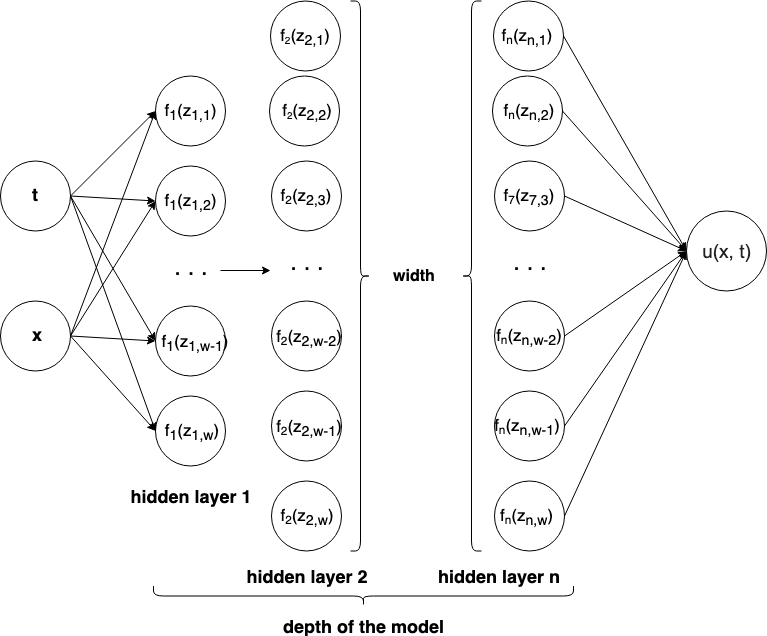
\includegraphics[width = 10cm , height = 7cm]{images/FFNN.png}
\\
\caption{Feed forward neural network.}
\end{figure}
\end{frame}

\begin{frame}{Why neural network is better than solving full PDE problem?}
Neural network must be evaluated only at the observation points\\
PDE problem must be computed on a grid, which includes observation points as a subset
\end{frame}

\begin{frame}{Neural network rough computational complexity}
    Let us denote $n^{(k)}$ the number of neurons in the $k$th layer, $L$ as the number of layers. Then the number of multiplications of weights is: $$n_{mul} = \sum_{k=2}^{L} n^{(k)}n^{(k-1)}n^{(k-2)} + n^{(1)}n^{(0)}*2.$$
    The number of activation function use is: $$n_g = \sum_{k = 1}^{L} n^{(k)}.$$     
    Then, we assume that matrices are quadratic and there the same number of neurons, and $L \sim n$:
    $$n_{mul} = L*n^3 \sim n^4, ~ n_g = L*n \sim n^2.$$
    Therefore, $ \text{ the computational complexity is: }  n_{mul} + n_g \sim O(n^4) + O(n^2) \Longleftrightarrow O(n^4).$ 
\end{frame}

\begin{frame}{Hyperparameter $\gamma$ is chosen via $K$-fold cross-validation}
\begin{equation*}
    \argmin_{\VLambda, \VTheta}
    \sum_{i=1}^N \big[ u_i - \UNN(x_i, t_i; \VTheta)\big ]^2 \enspace + \enspace
    \tikzmarkin<1->[set fill color=CRed, set border color=CRedD]{gamma}\gamma
    \tikzmarkend{gamma}
    \,
    \sum_{i=1}^N \big[ \FNN(x_i, t_i; \VLambda, \VTheta) \big]^2
\end{equation*}

Parameter $\gamma$ controls the balance between matching the data and satisfying
the model constraint.

\onslide<2>{
\begin{center}
\usebeamerfont*{frametitle}
How to choose the best $\gamma$?
\end{center}

Discretize $\gamma\in\R$ in some range and choose the
optimal value through the $K$-fold cross-validation.
}

\end{frame}

\begin{frame}{Hyperparameter $\gamma$ is chosen via $K$-fold cross-validation}
\begin{minipage}{\textwidth}
\centering
\begin{tikzpicture}[xscale=1.5, yscale=0.5, very thick]
    \node [scale=1] at (0.45, 1.6) {Validation};
    \draw [thick] (0.05, 1.05) -- (0.05, 1.15) -- (0.95, 1.15) -- (0.95, 1.05);
    \node [scale=1] at (3.0, 1.6) {Train};
    \draw [thick] (1.05, 1.05) -- (1.05, 1.15) -- (4.95, 1.15) -- (4.95, 1.05);

    \node [scale=1] at (-0.7, 0.5) {$k = 1$};
    \draw [fill=COrange] (0, 0) rectangle (1, 1);
    \draw                (1, 0) rectangle (2, 1);
    \draw                (2, 0) rectangle (3, 1);
    \draw                (3, 0) rectangle (4, 1);
    \draw                (4, 0) rectangle (5, 1);

    \node [scale=1] at (-0.7, -1.0) {$k = 2$};
    \draw                (0, -1.5) rectangle (1, -0.5);
    \draw [fill=COrange] (1, -1.5) rectangle (2, -0.5);
    \draw                (2, -1.5) rectangle (3, -0.5);
    \draw                (3, -1.5) rectangle (4, -0.5);
    \draw                (4, -1.5) rectangle (5, -0.5);

    \node [scale=1] at (1.5, -2.0) {$\dots \qquad \qquad \dots \qquad \qquad \dots$};

    \node [scale=1] at (-0.7, -3.0) {$k = K$};
    \draw                (0, -3.5) rectangle (1, -2.5);
    \draw                (1, -3.5) rectangle (2, -2.5);
    \draw                (2, -3.5) rectangle (3, -2.5);
    \draw                (3, -3.5) rectangle (4, -2.5);
    \draw [fill=COrange] (4, -3.5) rectangle (5, -2.5);
\end{tikzpicture}
\end{minipage}

% \begin{columns}
%     \begin{column}{0.48\textwidth}
%     For given $\gamma$:\\
%     1. Split the data in $K = 5$ folds\\
%     \vspace{0.5cm}
%     \end{column}
%     \begin{column}{0.48\textwidth}
%     2. Repeat $k$ times for a given $\gamma$: \\
%         \quad - train the neural network on ``white'' folds\\
%         \quad - compute prediction error on ``orange'' fold\\
%         \quad - average the results over all $K$ folds.\\
%     \vspace{0.5cm}
%     3. Repeat for discrete $\gamma$ in some range.
%     3) Choose the result with the least MSE.
%     \end{column}
% \end{columns}
\vspace{0.5cm}
\begin{columns}
    \begin{column}{0.3\textwidth}
        For given $\gamma$ in some range:
    \end{column}
    \begin{column}{0.7\textwidth}
        \begin{enumerate}
        \item Split the data in $K = 5$ folds
        \item Repeat $K$ times:\
            \begin{itemize}
            \item train the neural network on ``white'' folds
            \item compute prediction error on ``orange'' fold
            \end{itemize}
        \item Average the errors over $K$ folds
        \end{enumerate}
    \end{column}
\end{columns}

\vspace{0.4cm}
\textbf{In the end:} choose $\gamma$ with the minimal averaged prediction error.
\end{frame}

\begin{frame}{Bootstrapping parameters $\vec{\lambda}$}
    In this work, model parameter $\vec{\lambda}$ is estimated using bootstrap technique:\\
    \vspace{0.5cm}
    \quad - Set training and test data.\\
    Repeat for a several times $T$ the following steps:\\
    \quad - Choose 80\% of the sample data and use it for training and testing the model. \\
    \quad - Store the resulting $\vec{\lambda}$.\\
    \vspace{0.5cm}
    Results of bootstrap are given below for each problem.
\end{frame}

\begin{frame}{We use Tensorflow for all computations}
\begin{itemize}
    \item You specify functions as computational graphs
    \item It allows to compute derivatives automatically
    \item Can compute on videocards (it is faster than usual
          processors)
    \item Very useful for neural networks
\end{itemize}
    
\centering
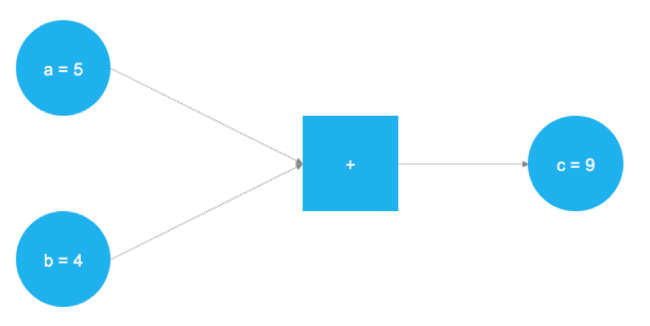
\includegraphics[scale = 0.2]{images/graph-example.png}
\end{frame}


% Common part (end)
% ------------------------------------------------------------------------------


% ------------------------------------------------------------------------------
% Heat equation part

\section{Example 1. Heat equation}

\begin{frame}{Heat equation}
We consider the linear heat equation
\begin{align*}
    &u_t - {\color{red}\lambda} u_{xx} - g(x, t) = 0, \quad x\in[-1; 1], \quad t\in[0, 1] \\
    &u(x, 0) = 0 \\
    &u(0, t) = u(1, t) = 0
\end{align*}
with source term $g(x, t) = (4\pi^2 -1) \, \sin(2\pi x) \, \exp(-t)$

\vspace{0.5cm}
True $\lambda$ is 1

Exact solution: $\quad u = \sin(2\pi x) \, \exp(-t)$
\end{frame}

\begin{frame}{Observations}
1. Compute $u$ on the uniform grid with $201\times101$ points in $x\times t$\\
2. Network complexity [2, 20, 20, 1]: 2 hidden layers with 20 neurons in each\\
3. In total $2\times20 + 20 + 20\times20 + 20 + 20\times1+1=501$ parameters in $\VTheta$\\
4. Sample 6400 observations uniformly\\
5. Large number of observations allows to avoid overfitting
\end{frame}

\begin{frame}{Observations}

\centering
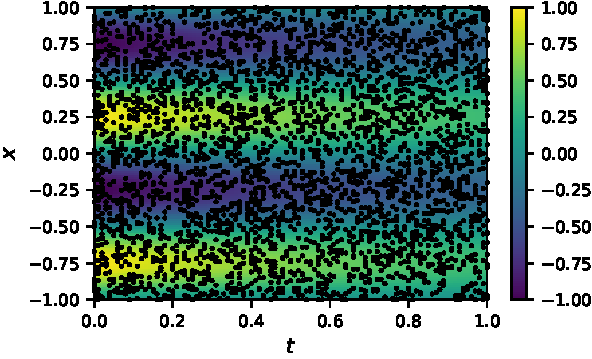
\includegraphics{images/heateq-observations}
\end{frame}

\begin{frame}{Cross-validation for $\gamma$}
\centering
Clean data: just exact solution

\vspace{0.5cm}
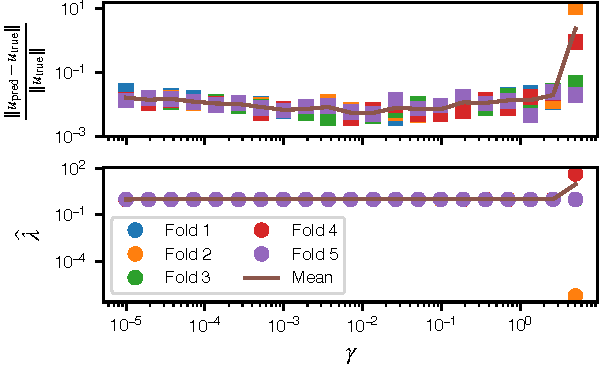
\includegraphics{images/heateq-cross_validation-clean}

\uncover<2->{
\begin{tikzpicture}[remember picture, overlay]
\node[yshift=1.5cm, above] at (current page.center) (txt) {$\gamma^* \approx \num{1.36e-2}$};
\draw [CRedD, ->, very thick] (txt) -- (1.2, 5.4);
\end{tikzpicture}
}
\end{frame}

\begin{frame}[label=current]{Cross-validation for $\gamma$, noisy observations}
\centering
Noisy data: $\quad u_{\text{obs}} = u +  N(0, \sigma^2), \quad \sigma=0.05u$

\vspace{0.5cm}
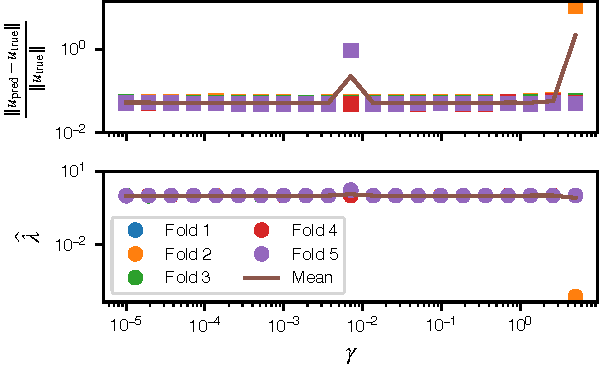
\includegraphics{images/heateq-cross_validation-noise}

\uncover<2->{
\begin{tikzpicture}[remember picture, overlay]
\node[xshift=2.7cm,yshift=1.5cm, above] at (current page.center) (txt)
    {$\gamma^* \approx \num{2.6}$};
\draw [CRedD, ->, very thick] (txt) -- (4.3, 5.5);
\end{tikzpicture}
}
\end{frame}

\begin{frame}{Uncertainty on $\widehat \lambda$ via bootstrap}
\begin{itemize}
    \item Both for clean and noisy data with corresponding optimal $\gamma$
    \item Simulate distribution of $\widehat \lambda$ via 100 values
    \item Detect and remove outliers via interquartile range method
    \item Compute bootstrap percentile intervals
\end{itemize}
\end{frame}

\begin{frame}{Uncertainty on $\widehat \lambda$ via bootstrap, clean data}
\centering
Clean data: just exact solution\\
Mean $\widehat \lambda \approx 1.0005$

\vspace{0.1cm}
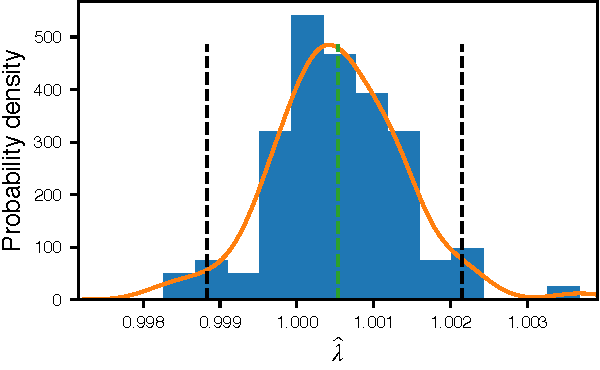
\includegraphics{images/heateq-bootstrap-clean}
\end{frame}

\begin{frame}{Uncertainty on $\widehat \lambda$ via bootstrap, noisy data}
\centering
Noisy data: $\quad u_{\text{obs}} = u +  N(0, \sigma^2), \quad \sigma=0.05u$\\
Mean $\widehat \lambda \approx 1.0052$ {\color{CRedD} (10x larger error than for clean data)}

\vspace{0.1cm}
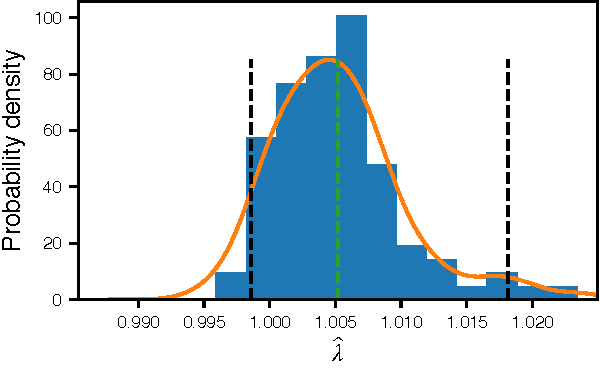
\includegraphics{images/heateq-bootstrap-noise}
\end{frame}

\begin{frame}{Predictions, clean data}
\centering
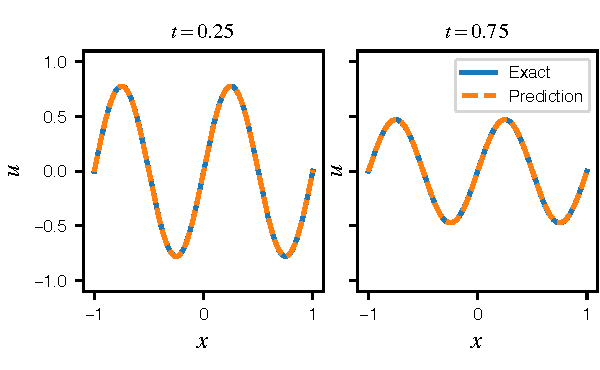
\includegraphics{images/heateq-predictions-clean}
\end{frame}

\begin{frame}{Predictions, noisy data}
\centering
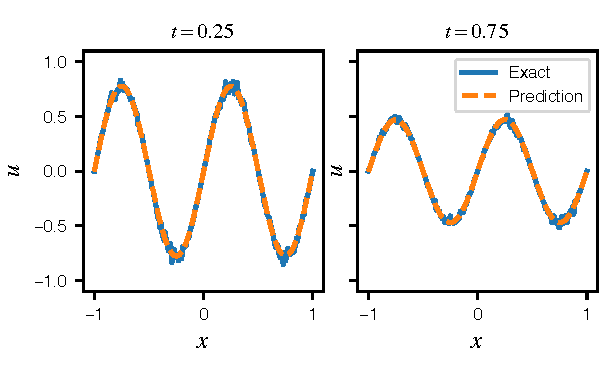
\includegraphics{images/heateq-predictions-noise}
\end{frame}

% Heat equation part (end)
% ------------------------------------------------------------------------------


% ------------------------------------------------------------------------------
% Burgers' equation

\section{Example 2. Burgers' equation}

\begin{frame}{Burgers' equation}
We consider the input data of the Burgers' equation:
\begin{align*}
&u_t + \lambda_1 u u_x - \lambda_2 u_{xx} = 0, \quad x\in[-1, 1], \quad t\in[0, T]\\
&u(0, x) = -\sin(\pi x) \\
&u(t, -1) = u(t, 1) = 0
\end{align*}

with true values of the sought-for parameters
\[
    \lambda_1 = 1,  \quad \lambda_2 = (0.01 / \pi) \approx 0.318.
\]

The exact solution is
$$u(t, x) = \frac{\pi \lambda_2}{\pi \lambda_2 e^{\{\pi^2 \lambda_2 t\}} - (e^{\{\pi^2 \lambda_2 t\}} - 1) cos(\pi x)}$$

\end{frame}

%\begin{frame}{Burgers' equation neural network configuration}
%    For this problem 3200 observations were used. The optimal
%number of them is: $2*M^2$, where $M$ is the number of model
%parameters. As we have 4 hidden layers with 10 neurons in each.
%This number basically affects the underfitting and overfitting
%of the neural network. \\

%    
%    The computational complexity according to the configuration
%of an NN consists of the number of matrix multiplications and
%the amount of the activation function use. 
    
%\end{frame}
\begin{frame}{Burgers' equation neural network configuration}
\begin{enumerate}
    \item The following network configuration was used:\\
$[2, 10, 10, 10, 10, 1]$.
    \item The number of the parameters in $\boldsymbol{\theta}$ is: \\
$2*10 + (10*10 + 10)*3 + 10*1 + 1 = 370$\\
    \item $3700$ observations were used.
\end{enumerate}

\end{frame}

\begin{frame}{Observations}
\small
Below, the exact solution is depicted on the uniform grid with 201 points in $x$ and 101 points in $t$. 
\begin{figure}
    \centering
    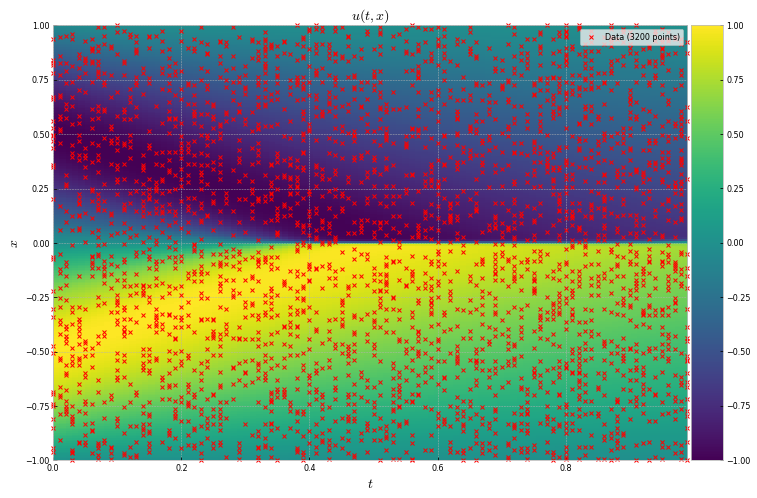
\includegraphics[width=10cm, height=6cm]{images/burgers-exact.png}
    \caption{The exact solution of Burgers' equation and 3200 observations.}
    \label{fig:my_label}
\end{figure}

\end{frame}

\begin{frame}

Hyperparameter $\gamma$ for the optimization problem was computed via cross-validation technique, using 5 folds. 

\centering
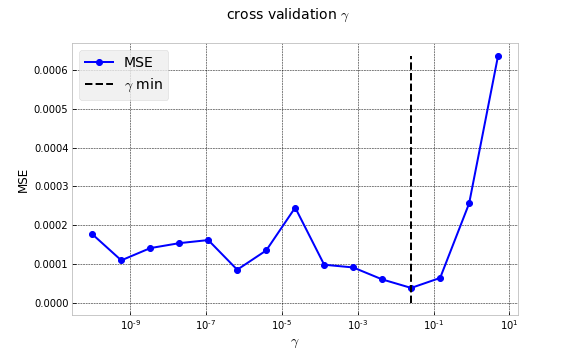
\includegraphics[width=11cm, height=7cm]{images/burgers-cross_val_gamma.png}

Cross-validation result for the hyperparameter $\gamma = 0.0255$.

\end{frame}

\begin{frame}

Parameter $\gamma$ for noisy data: $u_{obs} = u + N(0, \sigma^2),$

\centering
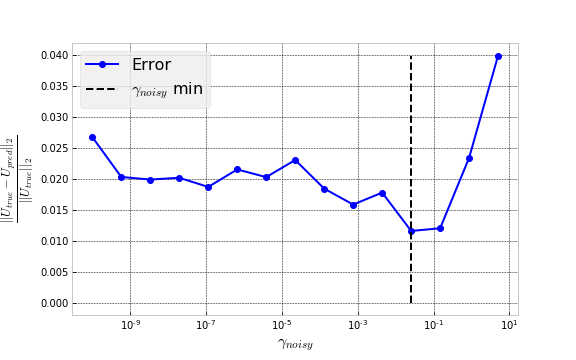
\includegraphics[width=11cm, height=7cm]{images/burgers-cross_val_gamma_noisy.png}\\

Cross-validation result for the hyperparameter $\gamma = 0.0255$ on the noisy data.

\end{frame}

\begin{frame}{Clean data results $\gamma=0.02553$}
Comparison between the exact and the predicted solutions at the different time instants t = 0.25, 0.50, 0.75. Training the network with $\gamma=0.0255$ gives prediction $\lambda_1 =
0.986564, ~ \lambda_2 = 0.00338$ with MSE $u(x, t) \approx 0.011 \,\%$.

\centering
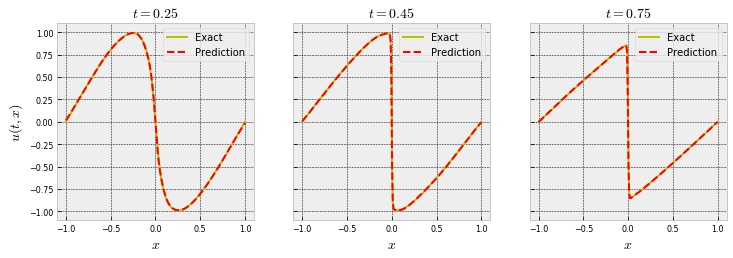
\includegraphics[scale=0.43]{images/burgers-exact-predict.png}


\end{frame}

\begin{frame}{Noisy data results}
Comparison between the exact and the predicted solutions for the noisy data. $u_{obs} = u + N(0, \sigma^2),$ \\

\centering
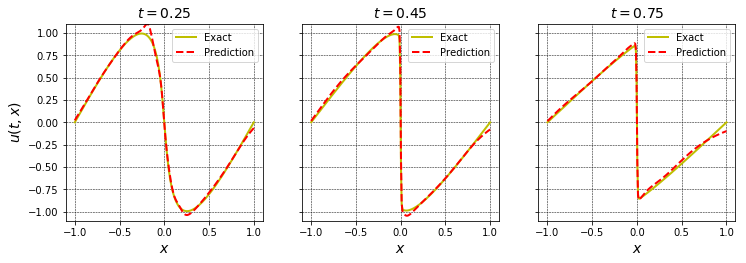
\includegraphics[scale = 0.43]{images/burgers-exact-pred-noisy.png}

Solution error $\frac{||U_{pred} - U_{true}||_2}{||U_{true}||_2}$ is: 47\%


\end{frame}

\begin{frame}{}

We have got the following bootstrapped results:

\centering
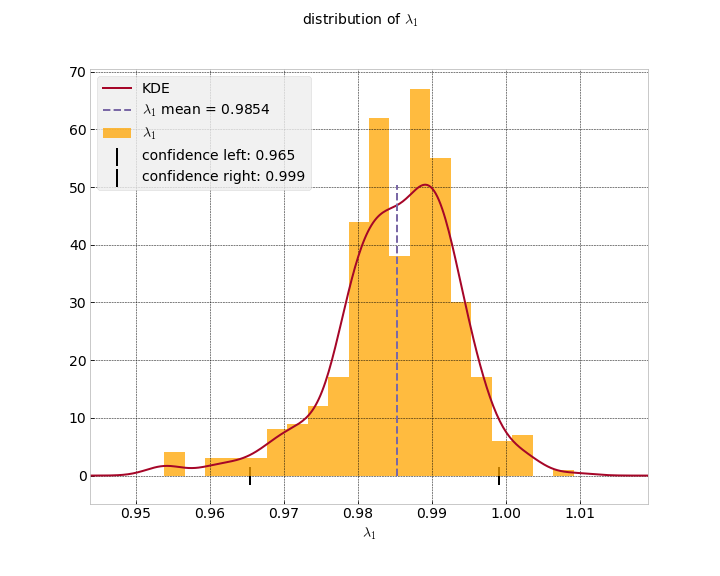
\includegraphics[width = 9cm , height = 7cm]{images/burgers-bootstraped_l1.png}

Bootstrapped parameter $\lambda_1$ for Burgers' equation.

\end{frame}

\begin{frame}

\centering
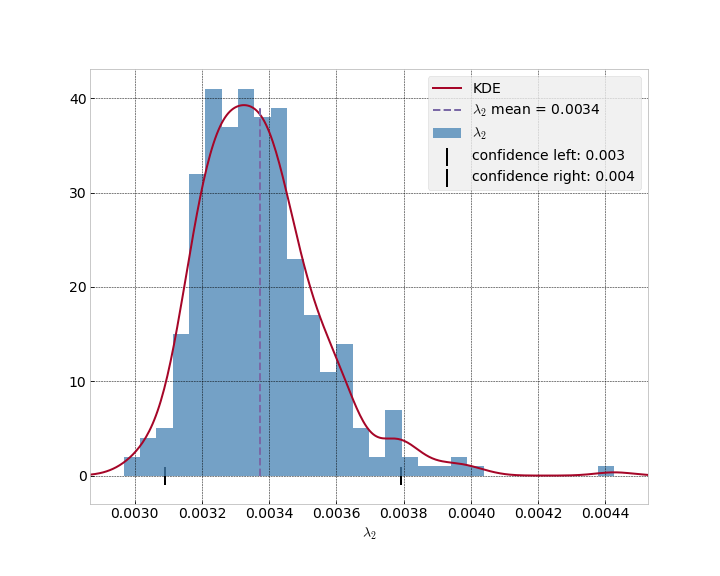
\includegraphics[width = 10cm , height = 8cm]{images/burgers-bootstraped_l2.png}

Bootstrapped parameter $\lambda_2$ for Burgers' equation.

\end{frame}

\begin{frame}{Neural Network configuration vs $\lambda$ error}

Below one can see the \% error in $\lambda_1$ and $\lambda_2$ for
different neural network configurations. In the first column the
number of the hidden layers is presented, in the second row the
number of the neurons in each hidden layer is presented.

\begin{tabular}{lccc|ccc}
    \toprule
    & \multicolumn{3}{c}{\% error in $\lambda_1$} & \multicolumn{3}{c}{\% error in $\lambda_2$}\\
  \midrule
%  \diagcell{.2em}{1.4cm}{\tiny{Layers}}{\tiny{Neurons}}
\diaghead{Columnmnm}{Layers}{Neurons} & 5 & 10 & 20 & 5 & 10 & 20 \\
\midrule
  1 & 19.43 & 31.82 & 25.32 & 118.02 & 79.2 & 74.33\\
  \hline
  2 & 24.93 & 8.75 & 3.21 & 56.05 & 28.35 & 23.48\\
  \hline
  4 & 3.42 & 0.82 & 0.29 & 13.56 & 2.43 & 4.21\\
  \hline
  6 & 3.26 & 2.16 & \textcolor{red}{1.29} & 19.53 & 2.79 & \textcolor{red}{0.66}\\
  \hline
  8 & 6.17 & 1.41 & 2.83 & 6.57 & 1.26 & 1.28\\
  \bottomrule
\end{tabular}

\end{frame}

\begin{frame}{Neural Network vs predicted solution error}

Below one can see the \% error in solution for different neural network configurations. 

\centering
    \begin{tabular}{lccc}
    \toprule
    & \multicolumn{3}{c}{\% error in solution $u(x, t)$} \\
    \midrule
    \diaghead{Columnmnm}{Layers}{Neurons}& 5 & 10 & 20  \\
    \hline
    1 & 19.16 & 15.98 & 13.45 \\
    \hline
    2 & 6.95 & 2.95 & 2.12 \\
    \hline
    4 & 1.53 & 1.05 & 0.74 \\
    \hline
    6 & 2.05 & 1.04 & \textcolor{red}{0.56} \\
    \hline
    8 & 2.61 & 0.84 & 0.91 \\
    \bottomrule
    \end{tabular}
    
    From the results above one can see that the optimal configuration of the model is: 6 hidden layers with 20 neurons in each.
\end{frame}

% Burgers' equation (end)
% ------------------------------------------------------------------------------

\begin{frame}{Conclusions}
    
\begin{itemize}
    \setlength\itemsep{0.75em}
    \item We apply neural networks to problem of parameter estimation.
    \item Adding physical constraint leads to efficient network training.
    \item Due to physical constraint, small number of observations works (small
          from neural-network point of view).
    \item Accurate estimates are reached with clean and noisy data.
    \item Parameter distributions look similar to normal distribution.
\end{itemize}

\end{frame}


\begin{frame}{Important references}
\begin{itemize}
    \setlength\itemsep{1.5em}
    \item Raissi, M., Perdikaris, P., \& Karniadakis, G. E. (2017). \emph{Physics informed deep learning (part II): Data-driven discovery of nonlinear partial differential equations}.\\
          \href{https://arxiv.org/pdf/1711.10566.pdf}{arXiv:1711.10566}
    \item Goodfellow, I., Bengio, Y., \& Courville, A. (2016). \emph{Deep learning}. MIT press.\\
          \url{http://www.deeplearningbook.org/}
    \item Hagan M. et al. (2014). \emph{Neural network design}. 2nd ed.\\
          \url{http://hagan.okstate.edu/nnd.html}
\end{itemize}
\end{frame}

\end{document}
